\documentclass[hyperref={pdftex}]{beamer}
\useoutertheme{shadow}
\usetheme{Madrid}
\usepackage{shortcuts}


\setbeamertemplate{section in toc}{\inserttocsectionnumber.~\inserttocsection}


\definecolor{mvablue}{rgb}{0.1098, 0.1373, 0.5137}
\definecolor{mvapurple}{rgb}{0.3373, 0.1529, 0.4510}
\definecolor{mvared}{rgb}{0.5725, 0.1882, 0.3922}

\colorlet{titleleft}{mvablue}
\colorlet{titlemiddle}{mvapurple}
\colorlet{titleright}{mvared}

\pgfdeclarehorizontalshading[titleleft,titlemiddle,titleright]
      {beamer@frametitleshade}{\paperheight}{
    color(0pt)=(titleleft);
    color(0.5\paperwidth)=(titlemiddle);
    color(\paperwidth)=(titleright)
  }

\renewcommand{\thefootnote}{\fnsymbol{footnote}}

\useinnertheme{tcolorbox}
\addtobeamertemplate{title}{
  \begingroup
  \tcbset{
    enhanced,
    interior style={left color=mvablue,right color=mvared}
  }
}{\endgroup}

\title{Deformable models and Geodesic Methods}
\subtitle{\textit{Automatic liver segmentation by integrating fully convolutional networks into active contour models}}

\author{Inès VATI\thanks{École Normale Supérieure Paris-Saclay, Master MVA}} %\thanks{ENS}
\institute[MVA]{
\includegraphics[height=1cm]{mva logo.png}}
\date{ \today } %\\  \vspace{0.3cm} \includegraphics[scale=0.2]{teaser.png}
\logo{
\includegraphics[width=0.6cm]{MVA-logo.png}}

% ---- Template -----
\setbeamercolor{author in head/foot}{parent=palette primary,bg=}
\setbeamercolor{title in head/foot}{parent=palette secondary,bg=}
\setbeamercolor{frame number}{parent=palette tertiary,bg=}

\makeatletter
\setbeamertemplate{footline}
{
    \leavevmode%
    \setbox\beamer@tempbox=\hbox{%
        \begin{beamercolorbox}[wd=.3\paperwidth,ht=2.25ex,dp=1ex,center]{author in head/foot}%
            \usebeamerfont{author in head/foot}\insertshortauthor\expandafter\beamer@ifempty\expandafter{\beamer@shortinstitute}{}{~~(\insertshortinstitute)}
        \end{beamercolorbox}%
        \begin{beamercolorbox}[wd=.4\paperwidth,ht=2.25ex,dp=1ex,center]{title in head/foot}%
            \usebeamerfont{title in head/foot}\insertshorttitle 
        \end{beamercolorbox}%
        \begin{beamercolorbox}[wd=.3\paperwidth,ht=2.25ex,dp=1ex,center]{frame number}%
         \usebeamerfont{frame number}\insertframenumber/\inserttotalframenumber
      \end{beamercolorbox}%
        }%
        \beamer@tempdim=\ht\beamer@tempbox%
        \advance\beamer@tempdim by 4pt%
        \begin{pgfpicture}{0pt}{0pt}{\paperwidth}{10pt}
            \pgfpathrectangle{\pgfpointorigin}{\pgfpoint{\paperwidth}{\beamer@tempdim}}
            \pgfusepath{clip}
            \pgftext[left,base]{\pgfuseshading{beamer@frametitleshade}}
        \end{pgfpicture}
        \vskip-\beamer@tempdim%
        \box\beamer@tempbox%    
}%
\makeatother
% -------------------
%% Table of content
\usepackage[style=authoryear]{biblatex}
\addbibresource{../report/ref.bib}

\AtBeginSection[] % \AtBeginSubsection
{
\begin{frame}{Overview}
\vfill
\tableofcontents[currentsection] % hideallsubsections
\vfill
\end{frame}
}

  
\newcommand{\myitem}{\item[$\rightarrow$]}
\newcommand{\mycoolitem}{\item[\checkmark]}

\begin{document}

% \frame[plain]{\titlepage}
\begin{frame}[plain]
  \titlepage
\end{frame}    

\begin{frame}{Table of contents}
  \tableofcontents
\end{frame}

% Presentation of the problem
\section{Problem statement}
\begin{frame}{Problem statement}
  \begin{itemize}
    \item Liver segmentation is a crucial step in liver surgery planning and monitoring
    \item Manual segmentation is time-consuming and prone to errors
    \item Accurate liver segmentation is a challenging task due to the liver's complex shape and the presence of other organs with similar intensities (stomach, heart)
  \end{itemize}
  \vfill
  \begin{center}
    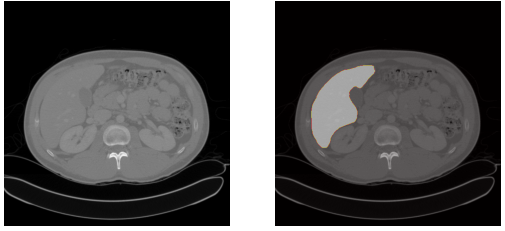
\includegraphics[width=.6\textwidth]{illu_liver_seg.png}
  \end{center}
\end{frame}

% Proposed methods
\section{Proposed Method}

\begin{frame}{Proposed Method}
 
    \textbf{Convolutional Neural Networks} $\rightarrow$ poor localization around object boundaries 
    
    \textbf{Active Contour Models} $\rightarrow$ sensitive to initialization, but topologically flexible

    \textbf{Integrated approach} $\rightarrow$ incorporating both high-level and low-level image information

    \vfill
    {\centering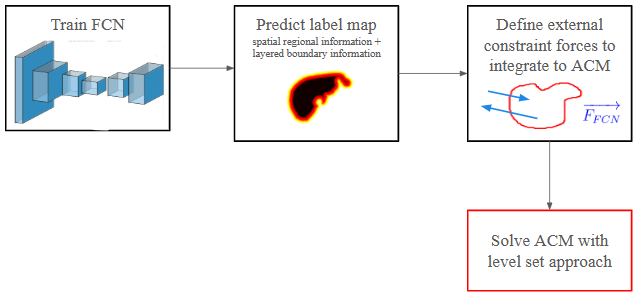
\includegraphics[width=.9\textwidth]{methods.png}}

    \citeall{guo_automatic_2019}
\end{frame}


\subsection{Generate layered label map containing rich information}
\begin{frame}{Generate layered label map containing rich information}
    \begin{columns}
        \begin{column}{.4\textwidth}
            For $7$ layers
            \begin{align*}
                L_{\blue{-3}} &= \lbrace X | \infty < \varphi(X) < -2.5 \delta \rbrace \\
                L_{\blue{-2}} &= \lbrace X | -2.5 \delta < \varphi(X) \leq -1.5 \delta \rbrace \\
                L_{\blue{-1}} &= \lbrace X | -1.5 \delta < \varphi(X) \leq -0.5 \delta \rbrace \\
                L_{0} &= \lbrace X | -0.5 \delta < \varphi(X) \leq 0.5 \delta \rbrace \\
                L_{\orange{1}} &= \lbrace X | 0.5 \delta < \varphi(X) \leq 1.5 \delta \rbrace \\
                L_{\orange{2}} &= \lbrace X | 1.5 \delta < \varphi(X) \leq 2.5 \delta \rbrace \\
                L_{\orange{3}} &= \lbrace X | 2.5 \delta < \varphi(X) \leq \infty \rbrace
            \end{align*}
            $\delta = d/\textrm{ps}$ is a parameter to control narrow bandwidth, $\textrm{ps}$ is the pixel spacing and $d$ is the bandwidth in millimeters
            \tiny{\grey{$d=5$}}
        \end{column}
    \hspace{.8cm}
    \begin{column}{.6\textwidth}
    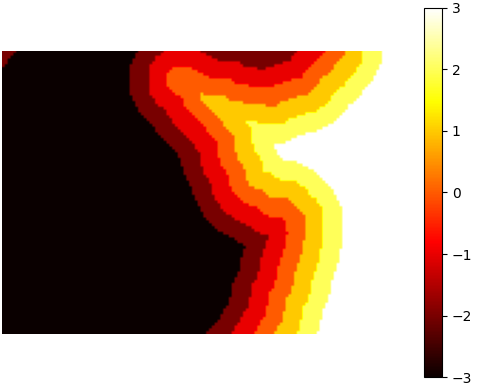
\includegraphics[width=.8\textwidth]{illu_layered_label_map.png}
    \end{column}
    \end{columns}
\end{frame}

\subsection{Train FCN to predict layered label map}
\begin{frame}{Train FCN to predict layered label map}
    Pre-trained model FCN-8 on the PASCAL dataset (21 classes)
     
    {\centering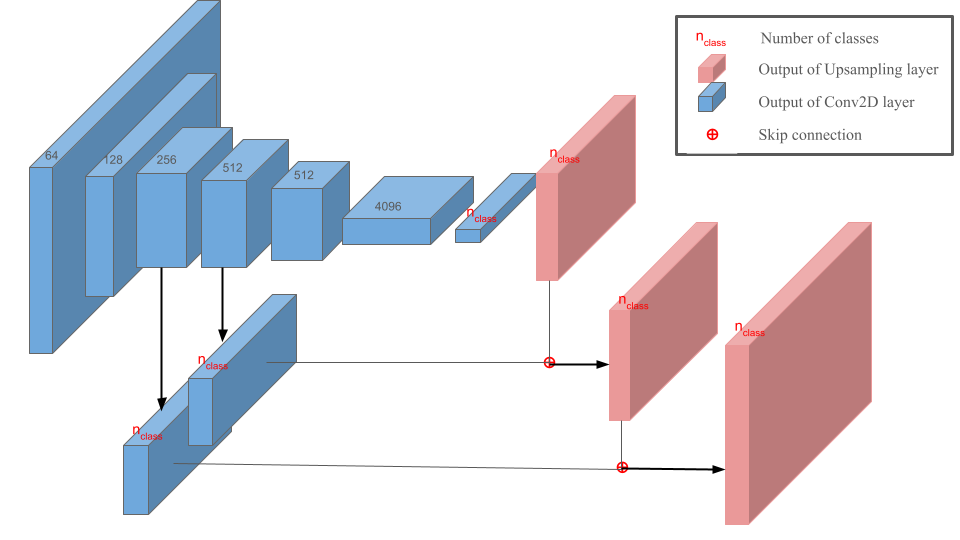
\includegraphics[width=\textwidth]{architecture.png}}
    \citeall{long_fully_2015}
\end{frame}

\subsection{Integrating NN's output to ACM}
\begin{frame}{Active Contour Models}
Let $\varphi$ be a Lipschitz function

Evolving the curve $C = \ens{(x, y)}{\varphi(x, y) = 0} $ in the normal direction with speed $V$ amount to solve 
$$
\left\lbrace \begin{array}{l}
    \frac{\partial \varphi}{\partial t} = V\norm{\nabla \varphi} \\
    \varphi(0, x, y) = \varphi_0(x, y) 
\end{array}
\right.
$$ 
$\varphi_0$ is the signed distance to the initial contour defined by the user

\citeall{chan_active_2001} 
\end{frame}

\section{Experiments and Implementation Details}
\subsection{Dataset}
\begin{frame}{CHAOS Dataset}
    \citeall{kavur_chaos_2019}
    \begin{itemize}
        \item $512 \times 512 $ CT images of 20 different patients with healthy liver (no tumor, lesions or any other diseases)
        \item For each patient, there is a series of DICOM images ($\sim$100 slices per patient)
        \item A dataset with challenges : partial volume effects, atypical liver shapes, etc.
    \end{itemize}
    % Partial volume effect is an artifact that occurs in CT scans when tissues of widely different absorption are encompassed on the same CT voxel, producing a beam attenuation proportional to the average value of these tissues

    \begin{figure}[H]
        \begin{subfigure}{.3\textwidth}
            \centering
            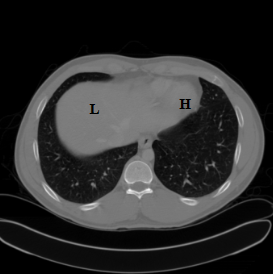
\includegraphics[width=\textwidth]{issues_ct1.png}
            \caption{Atypical shape}
        \end{subfigure}
        \begin{subfigure}{.3\textwidth}
            \centering
            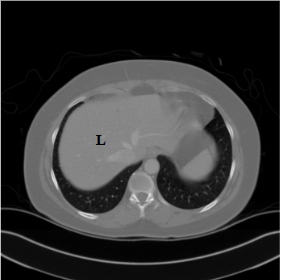
\includegraphics[width=\textwidth]{issue_ct2.png}
            \caption{Unclear boundary}
        \end{subfigure}
        \begin{subfigure}{.3\textwidth}
            \centering
            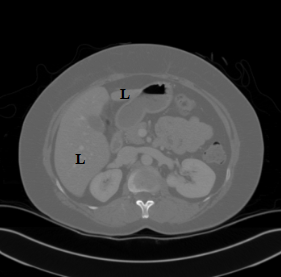
\includegraphics[width=\textwidth]{issue_ct3.png}
            \caption{Disconnected parts}
        \end{subfigure}
    \end{figure}
\end{frame}

\subsection{Train FCN}
\begin{frame}{Train FCN}
    Transfer learning with pre-trained FCN-8 weights from \citeauthor*{long_fully_2015}
    \begin{columns}
        \begin{column}{0.5\textwidth}
            \centering
            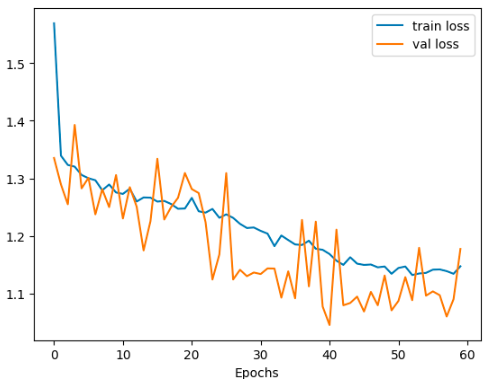
\includegraphics[width=\textwidth]{FCN8_pretrainedfreeze_lr0005_bs20_weights1x6-0.2.png} \\ 
            (1) Train only the new layers \\
            \tiny{\grey{Batch size of $20$, use of Cosine Annealing Learning Rate Scheduler from lr $= 0.005$}}
        \end{column}

        \begin{column}{.5\textwidth}
            \centering
            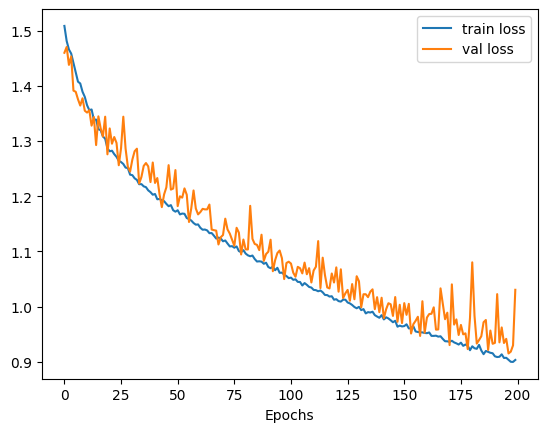
\includegraphics[width=\textwidth]{FCN8_pretrainedunfreeze.png} \\ 
            (2) Unfreeze some pre-trained layers {\tiny(the last 9)} \\
            \tiny{\grey{Batch size of $16$, lr $= 0.0001$}}
        \end{column}
    \end{columns}
    \vfill
    \grey{$2005$ training images, $200$ epochs, SGD optimizer with momentum of $.9$} \\ 
    The early stopper was never reached
\end{frame}

\subsection{Solve ACM}
\begin{frame}{Level Set Resolution}

 $\frac{\partial \varphi}{\partial t} = G(\varphi) $
    \begin{algorithm}[H]
        \caption{Level Set Method}
        \begin{algorithmic}
            \Input 
            \Desc{$I$}{(Normalized) Image}
            \Desc{$\varphi_0$}{Signed distance to the initial contour}
            \Desc{$N$}{Number of iterations} \Desc{$\delta t$}{Step size}
            \Desc{$n$}{Re-distancing period}
            \EndInput
            \State \textbf{Initialize} $\varphi^{(0)} \gets \varphi_0$
            \For{$t=0$ to $N$}
                \State Compute $G(\varphi^{(t)})$
                \State \magenta{$\varphi^{(t+1)} \gets \varphi^{(t)} - \delta t\ G(\varphi^{(t)})$} \Comment{Gradient Descent}
                \State Re-distancing $\varphi^{(t+1)}$ every $n$ iterations \Comment{Levelset Re-distancing} % :  computing the signed distance function to the zero level set
            \EndFor
        \end{algorithmic}
    \end{algorithm}
\end{frame}

\subsection{Comparative Analysis: Evaluating Active Contours Models}

\begin{frame}{Comparative Evaluation}
    \framesubtitle{Mean Curvature Motion with \magenta{global} regional Chan Vese forces}

    $$ G(\varphi) = \omega_0\norm{\nabla\varphi}\textrm{div}\left(\frac{\nabla \varphi}{\norm{\nabla\varphi}}\right) + \omega_1 ((I - c_{\textrm{ext}})^2 - (I - c_{\textrm{int}})^2 ) $$

    \begin{columns}
        \begin{column}{0.95\textwidth}    
        $$ c_{\textrm{int}} = \frac{\int_{\Omega}I(x)(1 - H(\varphi(x)))dx}{\int_\Omega 1 - H(\varphi(x)) dx} $$
        $$ c_{\textrm{ext}} = \frac{\int_{\Omega}I(x)H(\varphi(x))dx}{\int_\Omega H(\varphi(x)) dx} $$
        \end{column}
        \begin{column}{0.25\textwidth}
        \hspace*{-2cm}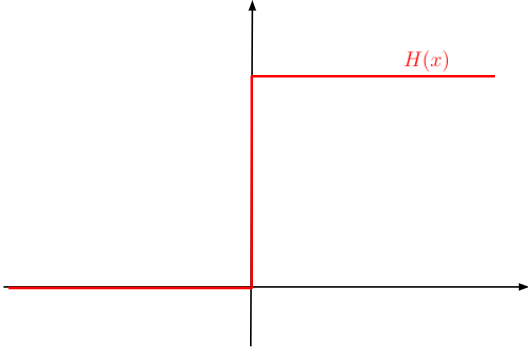
\includegraphics[width=\textwidth]{heaviside_func.png}
        \end{column}
    \end{columns}
    \vspace{0.7cm}
    \centering{\grey{\tiny 1000 iterations, $\omega_0=0.001$, $\omega_1=5$, $\delta t = 0.4$}}

    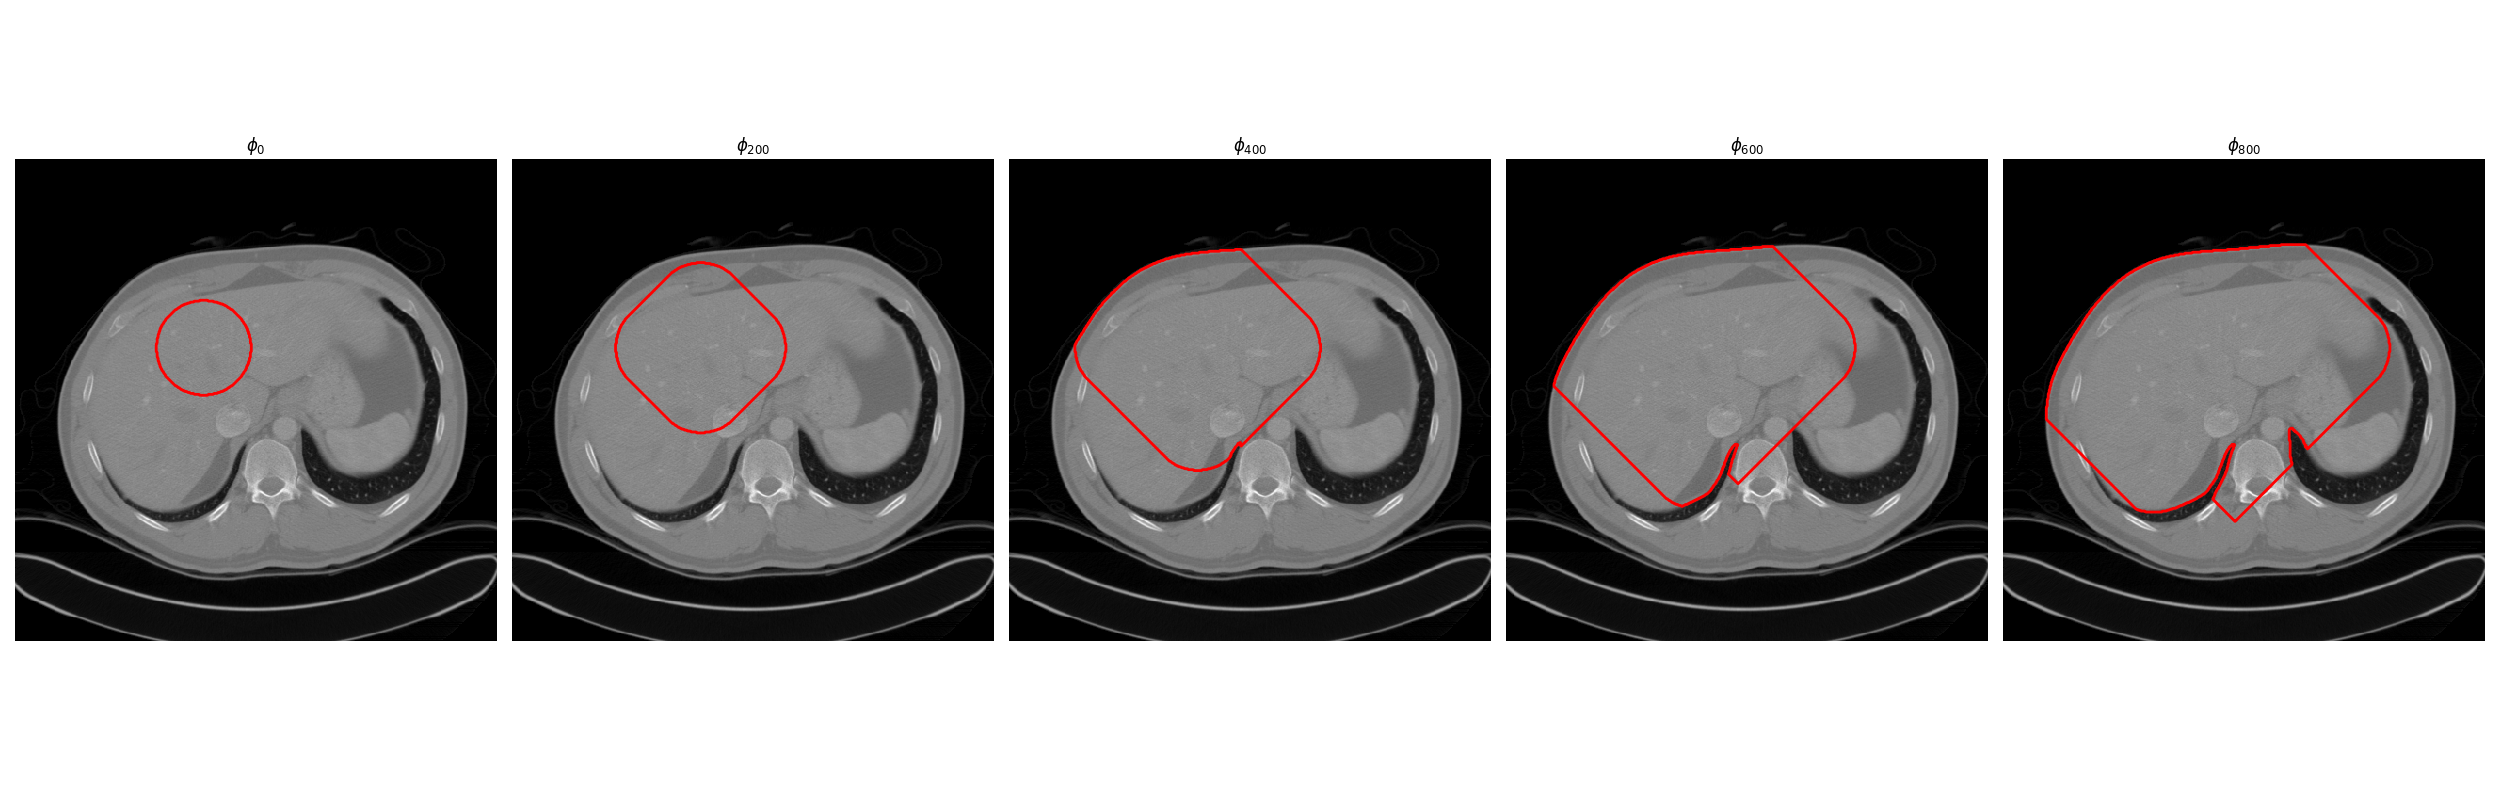
\includegraphics[width=\textwidth]{solve_acm__CVglobal_w[0.001, 0, 5]_FCNorder2.png}
\end{frame}

\begin{frame}{Comparative Evaluation}
    \framesubtitle{Mean Curvature Motion with \magenta{global} regional Chan Vese forces \magenta{with edge information}}
    \citeall{caselles_geodesic_1997}

    $$ G(\varphi) = \omega_0\magenta{g(I)}\norm{\nabla\varphi}\textrm{div}\left(\frac{\nabla \varphi}{\norm{\nabla\varphi}}\right) + \omega_0\dotp{\magenta{\nabla g}}{\nabla\varphi} +  \omega_1 F_{CV}  $$

    $$ g(I) = \frac{1}{\epsilon + \norm{\nabla\ k_\sigma * I}} $$


    \vspace{0.7cm}
    \centering{\tiny \grey{1000 iterations, $\omega_0=0.001$, $\omega_1=5$, $\delta t = 0.4$}}

    \includegraphics[width=\textwidth]{solve_acm__CVglobal_w[0.001, 0, 5]_FCNorder2_edgeinfo.png}
\end{frame}

\begin{frame}{Comparative Evaluation}
    \framesubtitle{Adding Edge Information}
    \citeall{caselles_geodesic_1997} 

    $$ W = g(I) = \frac{1}{\epsilon + \norm{\nabla\ k_\sigma * I}} $$
    \centering
    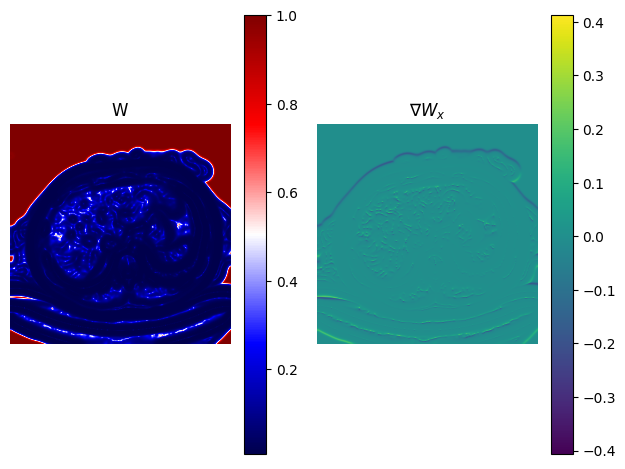
\includegraphics[height=.65\textheight]{edge_info.png}
\end{frame}

\begin{frame}{Comparative Evaluation}
    \framesubtitle{Mean Curvature Motion with \magenta{local} regional Chan Vese forces}
    \citeall{lankton_localizing_2008} 

    $$ G(\varphi) = \omega_0\norm{\nabla\varphi}\textrm{div}\left(\frac{\nabla \varphi}{\norm{\nabla\varphi}}\right) + \omega_1 ((I - c_{\textrm{ext}, x})^2 - (I - c_{\textrm{int}, x})^2 ) $$
    $$ B_r(x, y) = \ones_{\norm{x - y} \leq r}$$
    \begin{columns}
        \begin{column}{0.5\textwidth}
            $ c_{\textrm{int}, x} = \frac{\int_{\Omega}B_r(x, y)I(y)(1 - H(\varphi(y)))dy}{\int_\Omega B_r(x, y) (1 - H(\varphi(y))) dy} $
        \end{column}
        \begin{column}{.5\textwidth}
            $
            c_{\textrm{ext}, x} = \frac{\int_{\Omega}B_r(x, y)I(y)H(\varphi(y))dy}{\int_\Omega B_r(x, y) . H(\varphi(y)) dy}
            $
        \end{column}
    \end{columns}
    
    \vspace{0.4cm}
    \centering{\grey{\tiny 200 iterations, $\omega_0=0.1$, $\omega_1=5$, $\delta t = 0.4$, $r=10$}}

    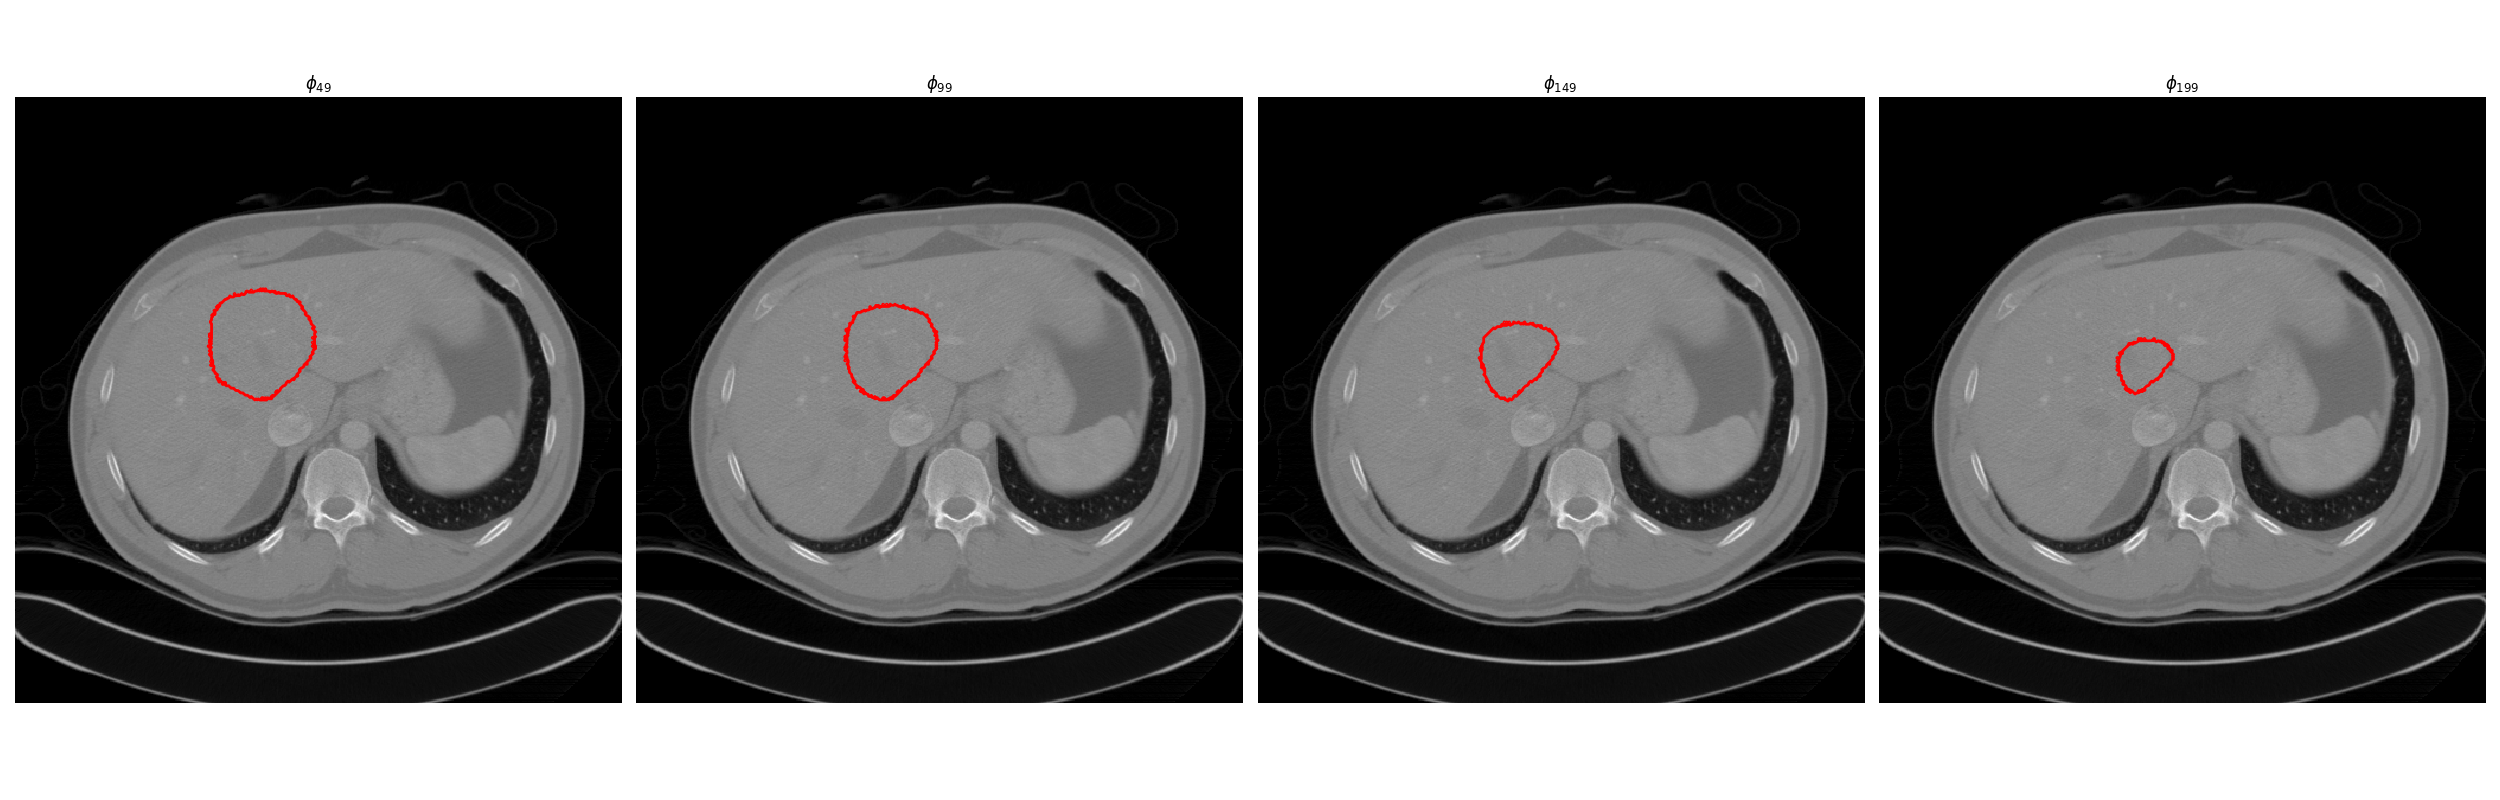
\includegraphics[width=\textwidth]{solve_acm__CVlocal_r10_w[0.1, 0, 5]_FCNorder2.png}
\end{frame}

\begin{frame}{Comparative Evaluation}
    \framesubtitle{Mean Curvature Motion with \magenta{local} regional Chan Vese forces \magenta{with edge information}}
    \citeall{caselles_geodesic_1997}

    $$ G(\varphi) = \omega_0\magenta{g(I)}\norm{\nabla\varphi}\textrm{div}\left(\frac{\nabla \varphi}{\norm{\nabla\varphi}}\right) + \omega_0\dotp{\magenta{\nabla g}}{\nabla\varphi} +  \omega_1 F_{CV,x}  $$

    $$ g(I) = \frac{1}{\epsilon + \norm{\nabla\ k_\sigma * I}} $$


    \vspace{0.7cm}
    \centering{\tiny \grey{1000 iterations, $\omega_0=0.1$, $\omega_1=5$, $\delta t = 0.4$, $r=10$}}

    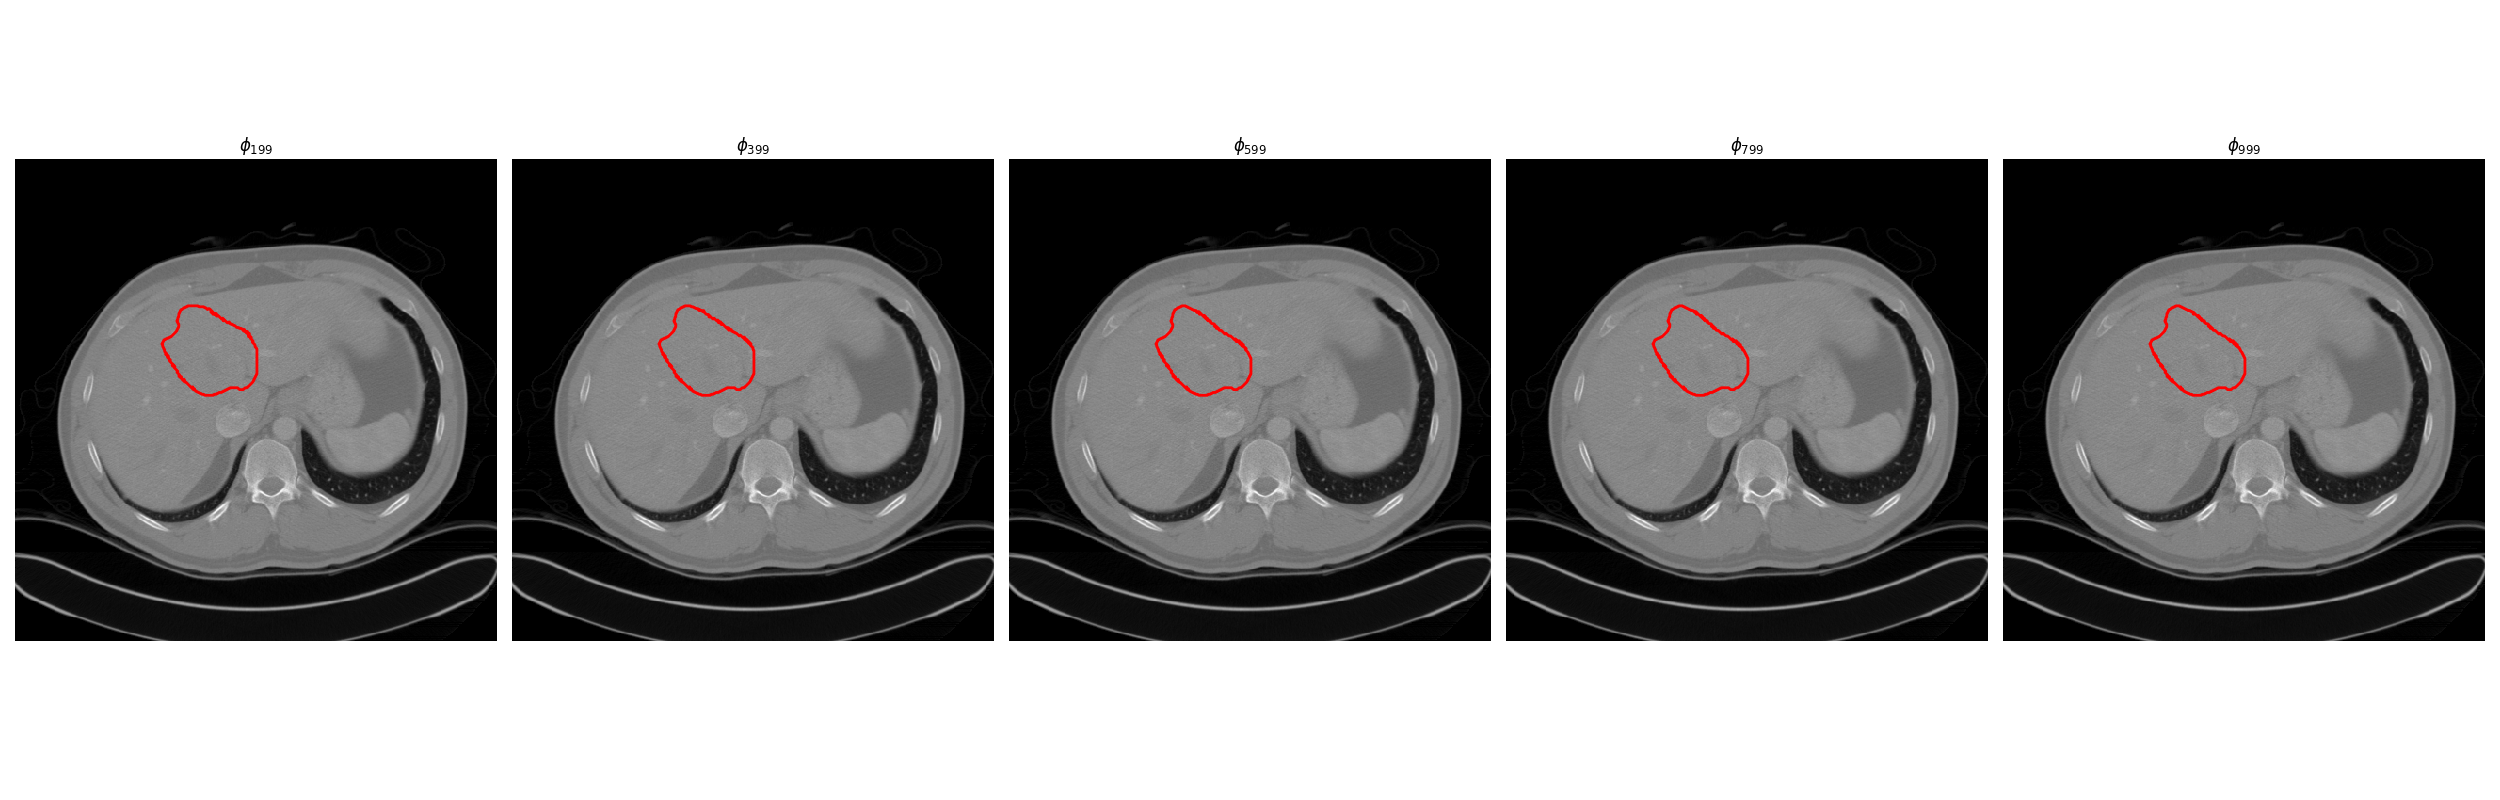
\includegraphics[width=\textwidth]{solve_acm__CVlocal_r10_w[0.1, 0, 5]_FCNorder2_edgeInfo.png}
\end{frame}

\begin{frame}{Comparative Evaluation}
    \framesubtitle{Mean Curvature Motion with \magenta{global} regional Chan Vese forces \magenta{with additional $F_{\textrm{FCN}}$}}
    \citeall{guo_automatic_2019} 

    $$ G(\varphi) = \omega_0 \norm{\nabla \varphi}\kappa + \omega_1F_{CV} + \omega_2 F_{\textrm{FCN}}$$
    \begin{columns}
        \begin{column}{.5\textwidth}
    Polynomial formulation of order $p$
    $ F_{\textrm{FCN}} = \textrm{sign}(L(x, y)) \abs{L(x, y)}^p \vec{n}$
        \end{column}
        \begin{column}{.5\textwidth}
            Exponential formulation
    $F_{\textrm{FCN}} = \alpha\ .\ \textrm{sign}(L(x, y)) \textrm{e}^{\abs{L(x, y)}}\vec{n}$
        \end{column}
    \end{columns}
    \vspace{0.7cm}
    \centering{\tiny \grey{1000 iterations, $\omega_0=0.01$, $\omega_1=5$, $\omega_2=1$, $\delta t = 0.4$, $p=2$}}
    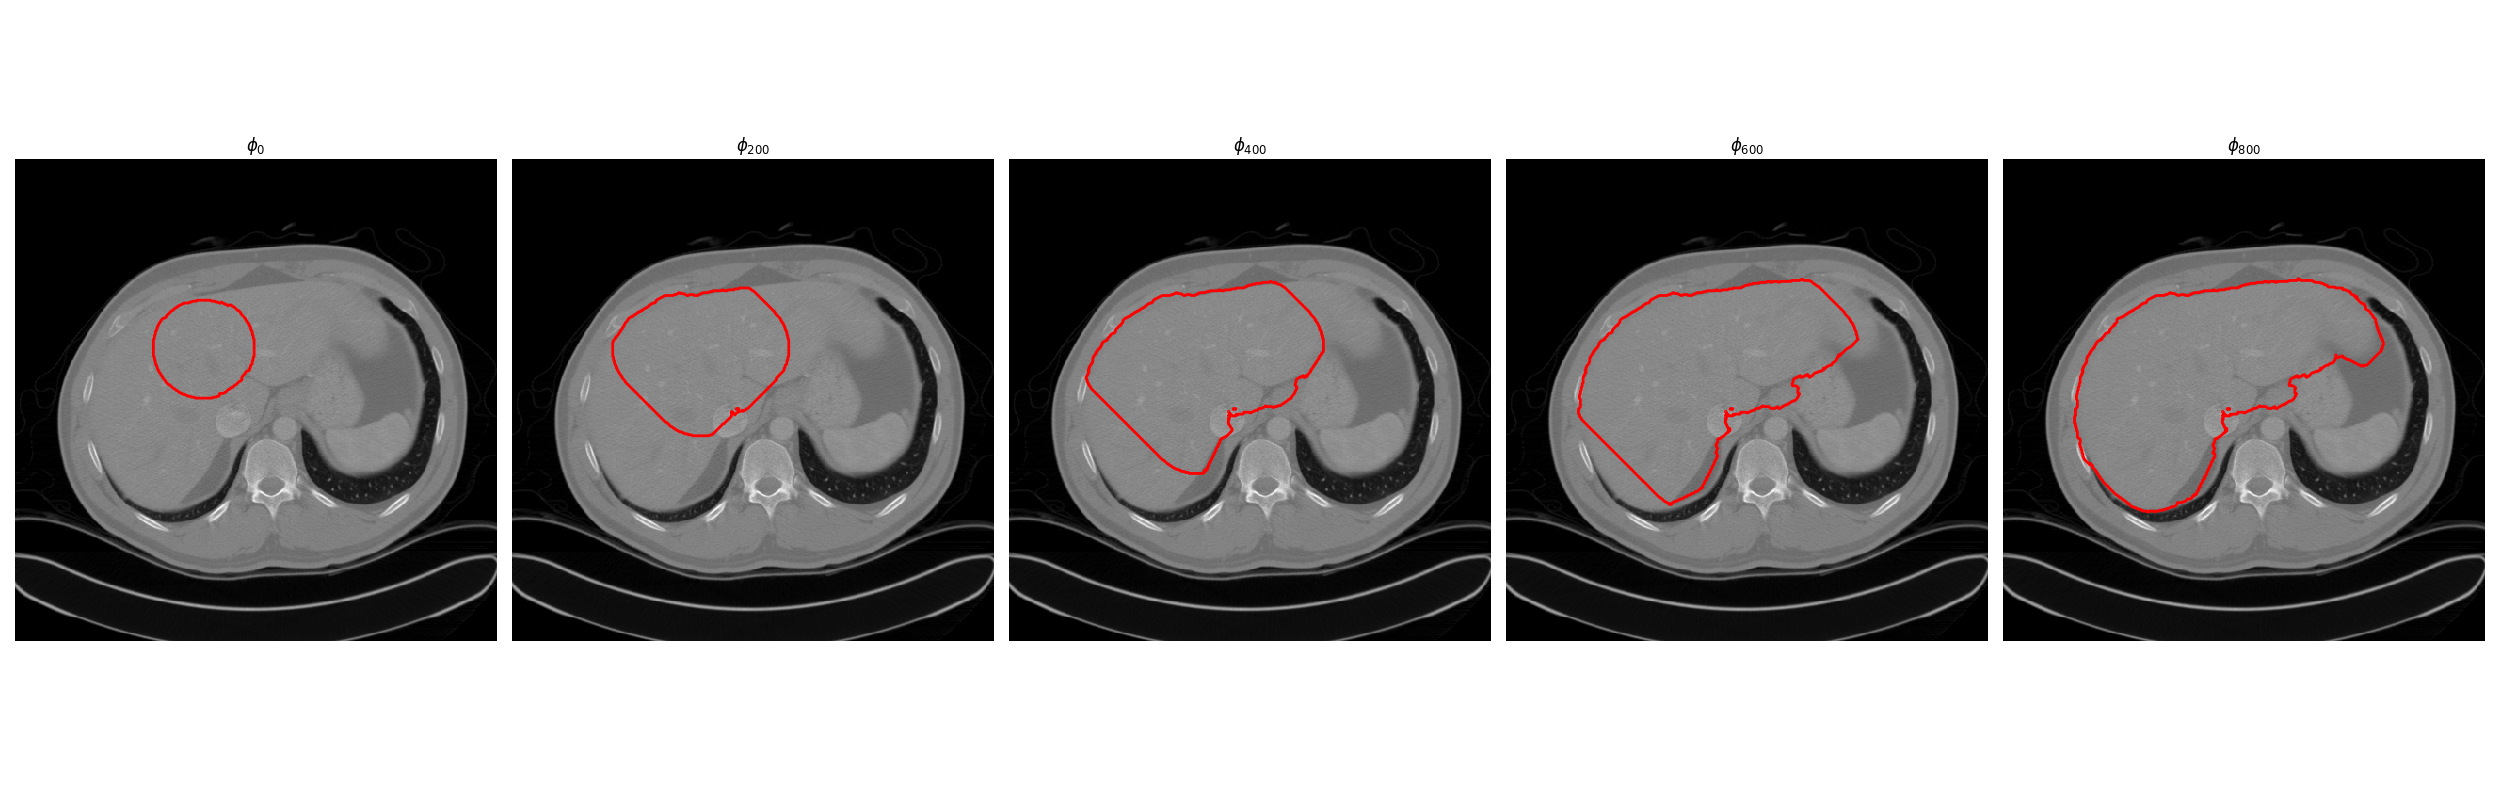
\includegraphics[width=\textwidth]{solve_acm__CVglobal_w[0.01, 1, 5]_FCNorder2.png}
    
\end{frame}

\begin{frame}{Comparative Evaluation}
    \framesubtitle{External constraint $F_{\textrm{FCN}}$ forces}

    \begin{center}
    \tiny \grey{Polynomial function with $p=2$} 

    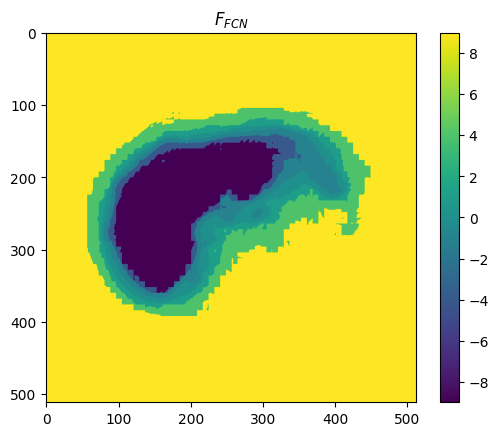
\includegraphics[height=.8\textheight]{f_fcn.png}
    \end{center}

\end{frame}

\begin{frame}{Comparative Evaluation}
    \framesubtitle{Mean Curvature Motion with \magenta{local} regional Chan Vese forces \magenta{with additional $F_{\textrm{FCN}}$}}

    $$ G(\varphi) = \omega_0 \norm{\nabla \varphi}\kappa + \omega_1F_{CV, x} + \omega_2 F_{\textrm{FCN}}$$

    \vspace{0.7cm}
    \centering{\tiny \grey{1000 iterations, $\omega_0=0.01$, $\omega_1=5$, $\omega_2=1$, $\delta t = 0.4$, $r=10$, $p=2$}}
    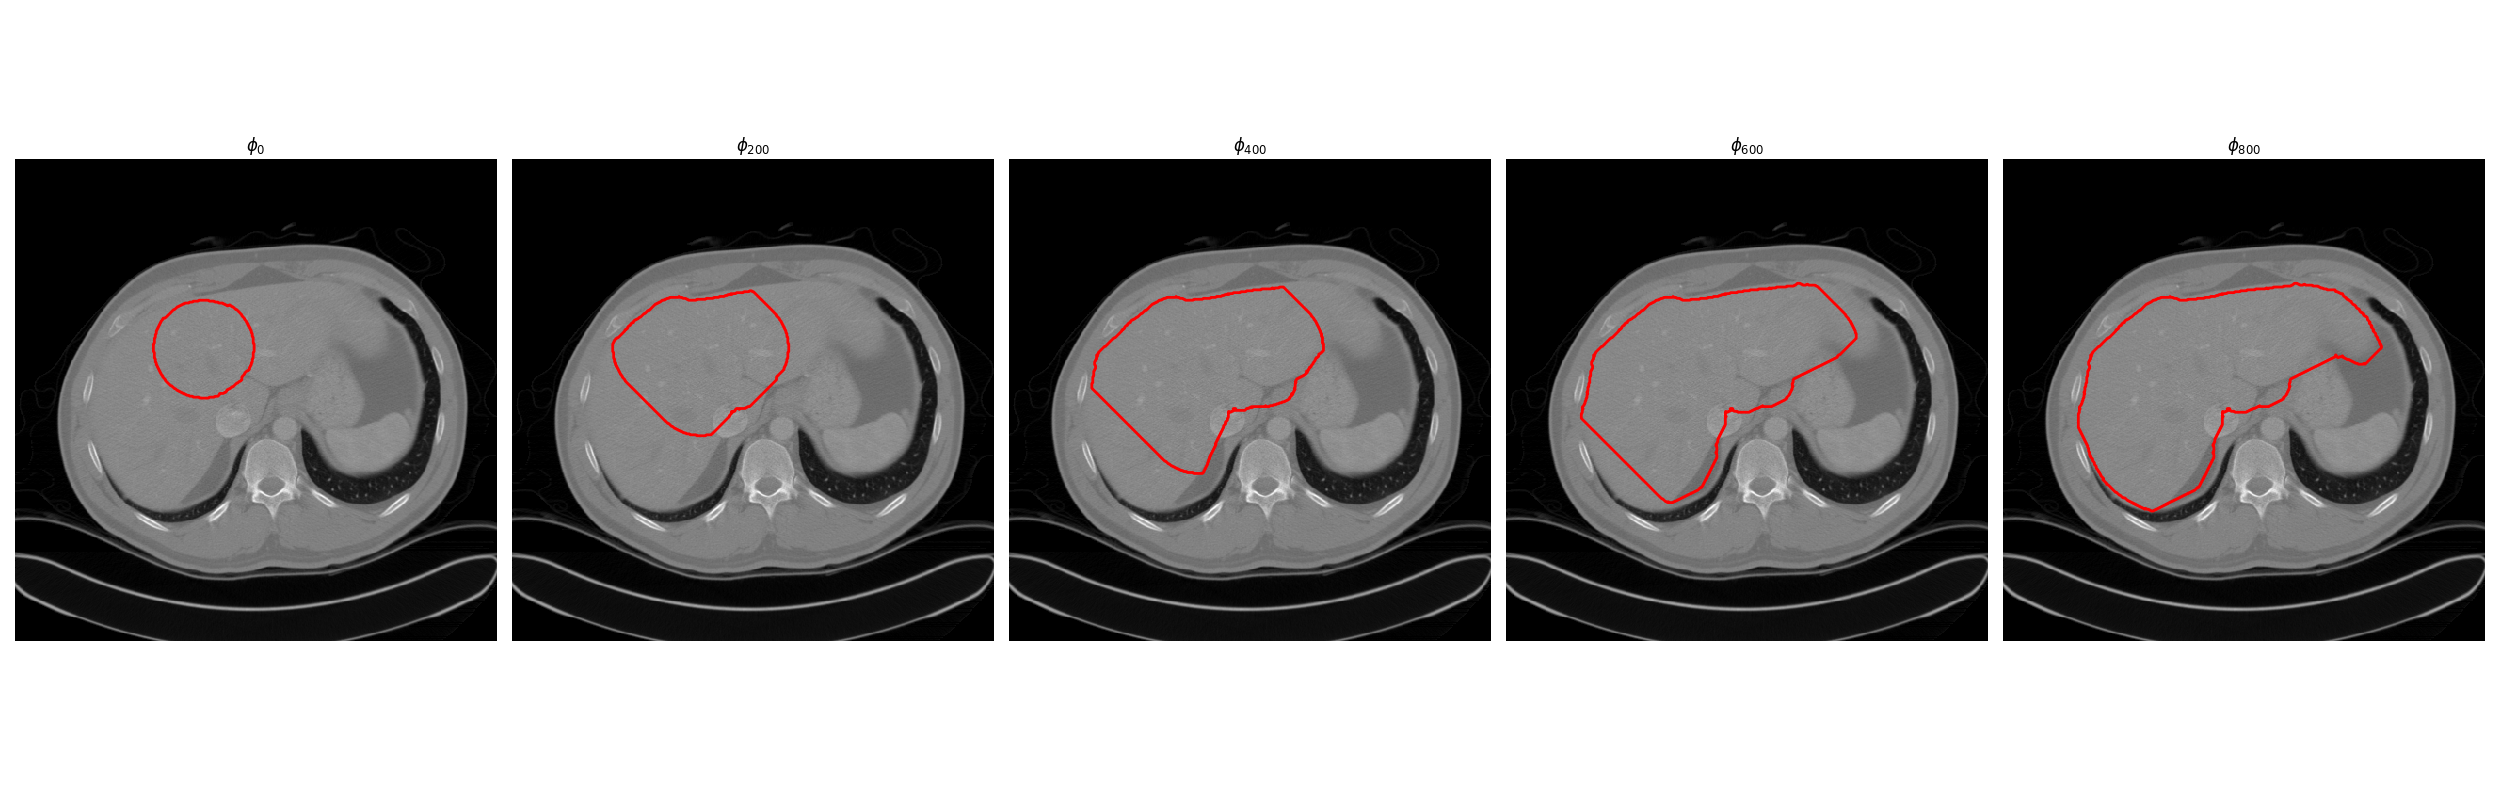
\includegraphics[width=\textwidth]{solve_acm__CVlocal_w[0.01, 1, 5]_FCNorder2.png}
\end{frame}

\subsection{A Pathological Case}
\begin{frame}{A Pathological Case}
    \centering
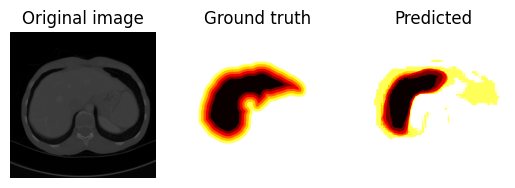
\includegraphics[height=.45\textheight]{ex_bad_case.png}
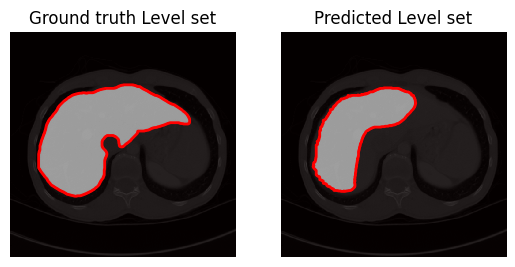
\includegraphics[height=.5\textheight]{ex_bad_case_levelset.png}
\end{frame}

\begin{frame}{A Pathological Case - Result}
    Mean Curvature Motion with global Chan Vese forces and polynomial FCN forces \\ 
    \centering{\tiny \grey{1000 iterations, $\omega_0=0.01$, $\omega_1=5$, $\omega_2=1$, $\delta t = 0.4$, $p=2$}} 

    \centering
    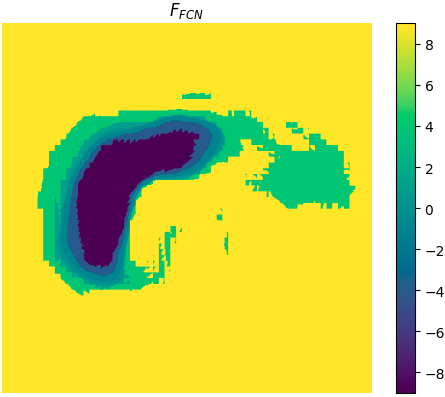
\includegraphics[height=.4\textheight]{bad_case_f_fcn.png}
    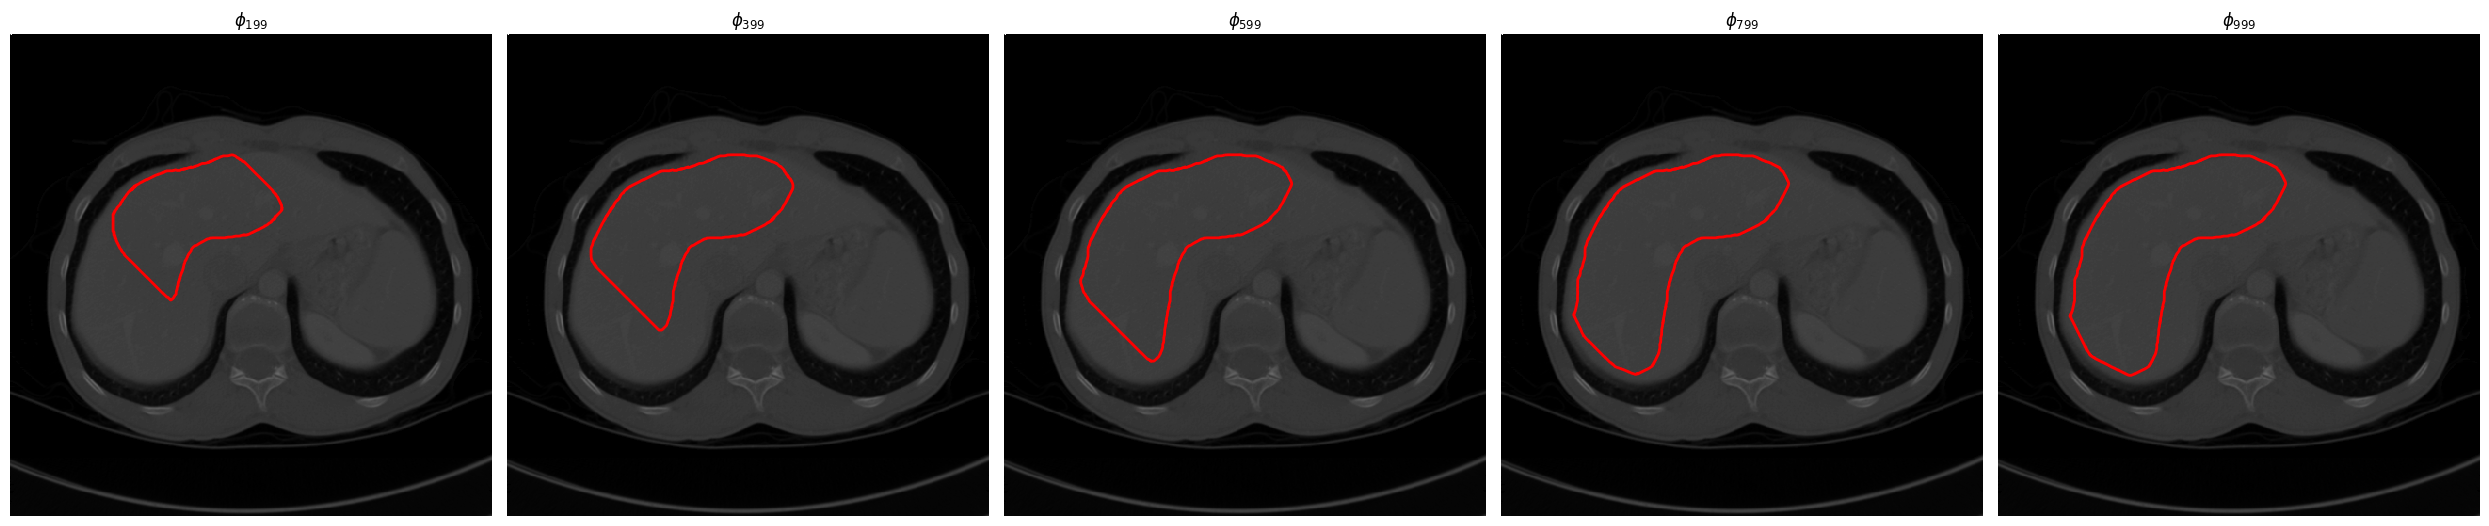
\includegraphics[width=\textwidth]{bad_case__CVglobal__w[0.01, 0.5, 5]_FCNorder2.png}
\end{frame}


% Critics
% Conclusion / perspective
\section{Conclusion and Perspectives}
\begin{frame}{Conclusion and Perspectives}
  \begin{itemize}
    \item Parallel with the Balloon model (inflation force)
    \item Possible improvements by using another method for level set Resolution : sparse field method [\citeonslide{guo_automatic_2019}, \citeonslide{whitaker_level-set_1998}]
    \item Train with additional dataset (SLIVER07)
    \item Experiment with other architectures (Other FCNs 
    [\citeonslide{long_fully_2015}], DeepLab [\citeonslide{ferrari_encoder-decoder_2018}], U-Net [\citeonslide{huang_unet_2020}])
\end{itemize}
\end{frame}

\begin{frame}[allowframebreaks]{References}
    \printbibliography
\end{frame}

\end{document}